\subsection{Zero-Shot Model (Flan-T5)}

\begin{figure}[H]
  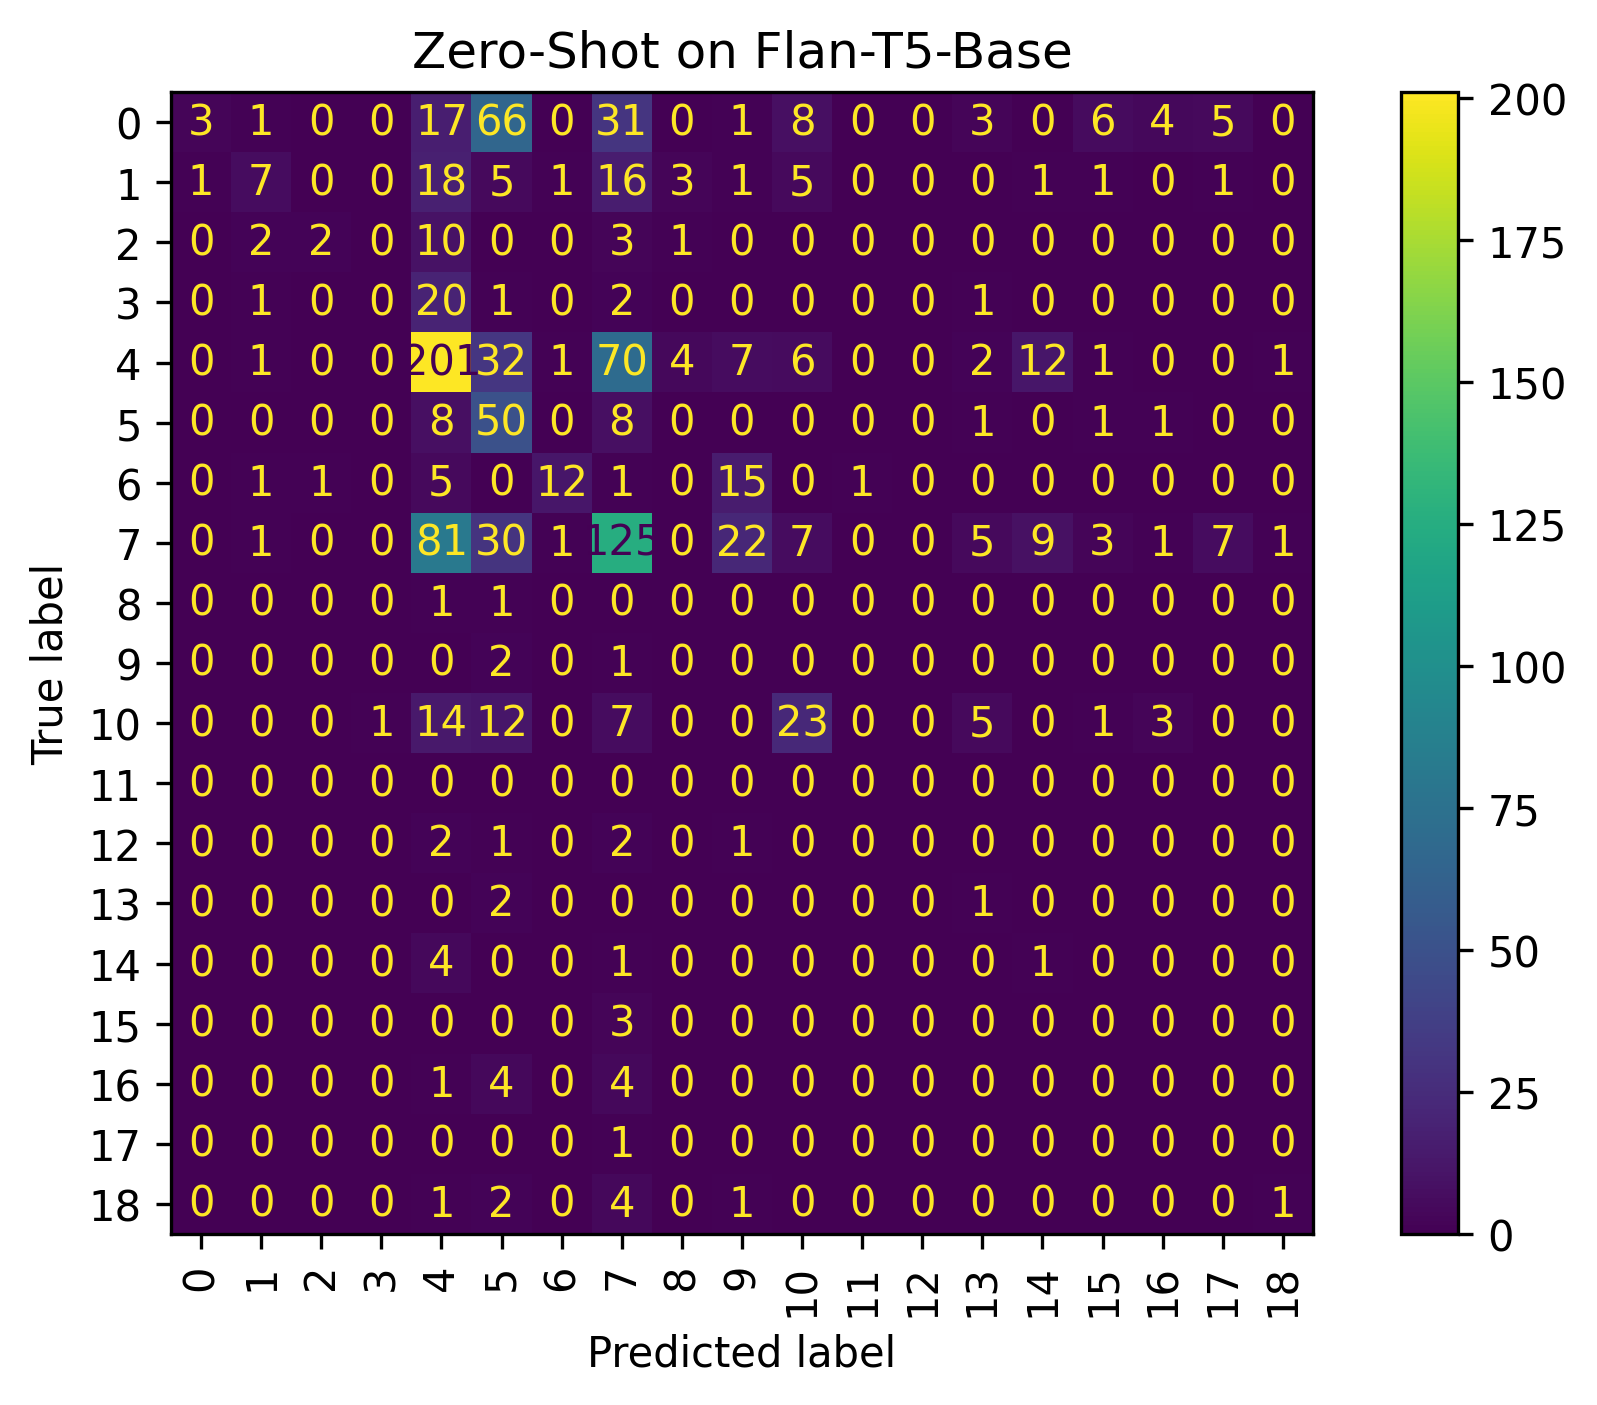
\includegraphics[width=\columnwidth]{Dan/Images/confusion_matrices.png}
  \caption{Confusion matrix for Zero-shot Model (Flan-T5-Base).}
  \label{fig:zscf}
\end{figure}

Analyzing Figure~\ref{fig:zscf}, the model appears to be best at identifying comedy and drama descriptions, but still struggles with differentiating between the two. 
Many descriptions are misclassified as crime, film-noir, and romance. 
Action is especially confused with crime and drama, which may be because there is a high overlap in the vocabulary between these classes. 
In addition, many instances are misclassified as film-noir despite the class being relatively infrequent in the dataset, which may indicate the model does not have a clear grasp on what the token actually represents, e.g. its training corpus neglects the term.

